%%%%%%%%%%%%%%%%%%%%%%%%%%%%%%%%%%%%%%%%%%%%%%
%                insertmeeting
% 1) Title (something creative & funny?)
% 2) Date (MM/DD/YYYY)
% 3) Location (ex. Hagerty High School)
% 4) People/Committees Present 
% 5) Picture 
% 6) Start Time & Stop Time (ex. 12:30AM to 4:30PM)
%%%%%%%%%%%%%%%%%%%%%%%%%%%%%%%%%%%%%%%%%%%%%%
\insertmeeting 
	{Scrappy Scrimmaging} 
	{11/02/21}
	{Hagerty High School}
	{Annika, Anouska, Clayton, Falon, James, Jensen, Nathan, Ritam, Rose, Samantha, Lilly}
	{Images/RobotPics/robot.jpg}
	{2:30 - 4:30}
	
\hhscommittee{General}
\noindent\hfil\rule{\textwidth}{.4pt}\hfil
\subsubsection*{Goals}
\begin{itemize}
    \item Discuss goals and possibilities for our scrimmage, meet1, and beyond  

\end{itemize} 

\noindent\hfil\rule{\textwidth}{.4pt}\hfil

\subsubsection*{Accomplishments}
Because we have had lots of new ideas and designs in the past few weeks, we decided to meet as a team and discuss what was possible for us to complete in the next couple weeks before the meet and what we want to complete for next time. To start our discussion, we looked back at the competition planning schedule from right after kick-off, detailing many of the goals we had for the season (Figure \ref{fig:110221_1}). In looking at this spreadsheet, we noticed how much our ideas had changed and how far we had come, and we decided to make some changes to help us map out our new goals going forward. 
Of our goals for our scrimmage, which will be held this Thursday, the only one we haven't completed is parking in autonomous, but we are confident that in the next week, our software committee will be able to surpass this goal, though probably not by the scrimmage. 
Next, we shifted our attention to the much more important event: Meet 1. Of these goals, we have completed all, but making a team element. Although this hasn’t been completed, this is an important goal that needs to be accomplished. We have already made some progress on it by deciding on the color it needs to be: green because it has the most contrast with the rest of the field. The other goal that stuck out to us was having a vertical lift completed. Although this goal was never completed because we changed our strategy from having a vertical lift to having a pivoting arm, we still considered it complete because we have a way of picking up and scoring elements into both the shared and alliance shipping hubs. We all had a laugh at how different our robot robot has turned out from what we had originally planned and how shocked we would have been if we saw our current robot all the way back then! Seeing these differences, we changed our goals for meet one, adding having vision code and multiple autonomous programs. Overall We seem well on track for completing all of our goals for the first meet!
With all of our new ideas, we decided to look a bit farther into the future and amend our goals for meet 2 as well. The first goal that we wanted to add was concerning the intake. Because we have the double intake partially designed, we will push back its construction until after the first meeting to allow time for our software committee and drive team to work before meet 1. In the spreadsheet, we wrote “improve efficiency of intake” because although we have a design in cad, we still aren't sure what the final product of our new intake will look like. The other addition we made for meet 2 was to create odometry code. Like intake, this is something we started on but don’t want to add just a week before the competition. Still, we hope to have odometry up and running before meet 2. Because we aren't sure what the future will hold, we decided not to change our goals for anything past meet 2. Our edited sheet is shown below (Figure \ref{fig:110221_2}).

\begin{figure}[htp]
\centering
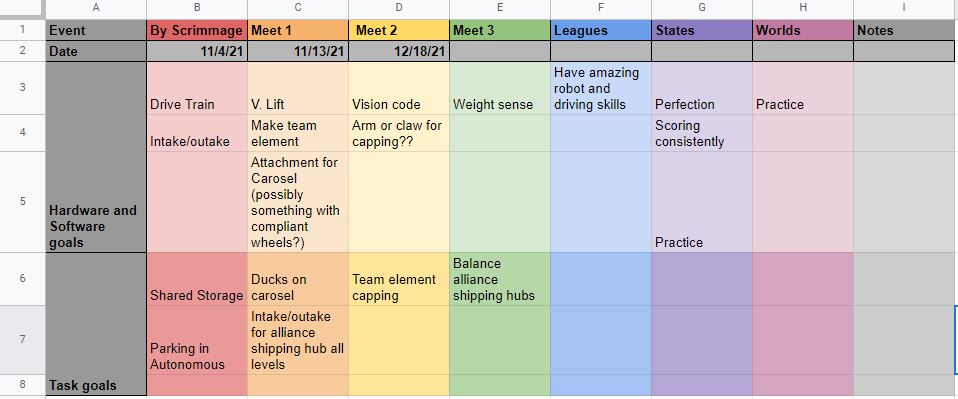
\includegraphics[width=0.95\textwidth, angle=0]{Meetings/November/11-02-21/11-2-21_Team_Figure1 - Nathan Forrer.JPG}
\caption{First draft of our goals}
\label{fig:110221_1}
\end{figure}
 

\begin{figure}[htp]
\centering
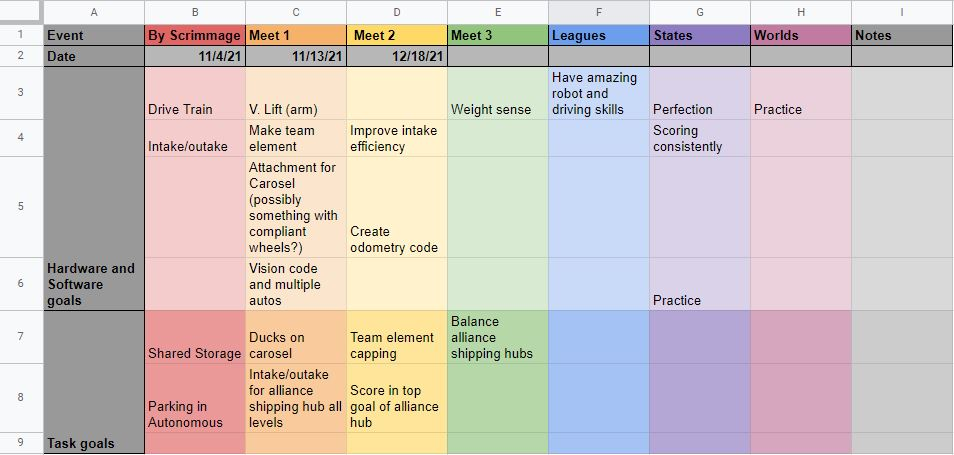
\includegraphics[width=0.95\textwidth, angle=0]{Meetings/November/11-02-21/11-2-21_Team_Figure2 - Nathan Forrer.JPG}
\caption{Edited goals}
\label{fig:110221_2}
\end{figure}

\hhscommittee{Software}
\noindent\hfil\rule{\textwidth}{.4pt}\hfil
\subsubsection*{Goals}
\begin{itemize}
    \item Add a program that takes a picture of the team element and critique the HSV in the code

\end{itemize} 

\noindent\hfil\rule{\textwidth}{.4pt}\hfil

\subsubsection*{Accomplishments}
During this meeting, we changed the hue, saturation, and value of the color the webcam would find so it would match the team element. To test if we found the correct color, we took a picture and had the code draw a bounding rectangle around the area the webcam found with the vision software. We included a Boolean that allows us to use just the vision software without running the autonomous. We were able to save the image and download it from Android Studio to see what it found. We added an If statement to find which level of the alliance shipping hub the block should be placed in autonomous based on the location of the team element. We printed the position of the left barcode and the middle barcode from the blue side onto the driver hub. We include the center between the middle and left barcodes by taking the average of the two numbers which is the barcode center. This allows us to use the X Center to find which barcode the team element is placed on. The X Center is the center of the rectangle that is placed around the team element. Since the placement of the robot on the field can only see two barcodes, the one not in the frame sets the X Center equal to zero. To differentiate between the other two barcodes, we choose whether the X Center is greater than or less than the barcode center. In each of the autonomous classes, there is an If statement that includes which level of the alliance hub it should go to based off the barcode position and the alliance. 


\whatsnext{
\begin{itemize}
    \item Test the robot in scrimmage
    \item Create autonomous code
    \item Practice driving before meet 1
    \item Start on a backup vision software
\end{itemize} 
}

